% Figure: scale covariance (A8) as a commuting square, with the scale axis relabelled.
% Referenced from §3.3. Pure TikZ. Paper I's fig-covariance-square with this article's letters
% (the dilation D_lambda of the line, the relabelling S_lambda, scales s <= t).

\begin{figure}[t]
\centering
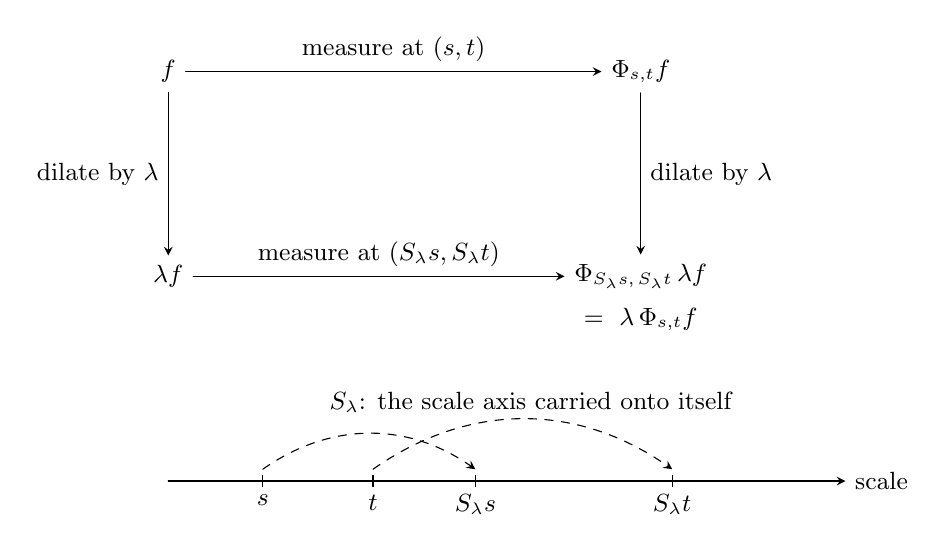
\begin{tikzpicture}[every node/.style={font=\small}, line cap=round, >=stealth]

% ---------- the commuting square ----------
\node (f)   at (0,2.6)   {$f$};
\node (Pf)  at (6.0,2.6) {$\Phi_{s,t} f$};
\node (Df)  at (0,0)     {$\Dil{\lambda} f$};
\node (PDf) at (6.0,0)   {$\Phi_{S_\lambda s,\,S_\lambda t}\,\Dil{\lambda} f$};
\node[anchor=north] at (PDf.south) {$=\ \Dil{\lambda}\,\Phi_{s,t} f$};

\draw[->] (f)  -- node[above] {measure at $(s,t)$} (Pf);
\draw[->] (f)  -- node[left]  {dilate by $\lambda$} (Df);
\draw[->] (Pf) -- node[right] {dilate by $\lambda$} (PDf);
\draw[->] (Df) -- node[above] {measure at $(S_\lambda s, S_\lambda t)$} (PDf);

% ---------- the scale axis, relabelled ----------
\begin{scope}[yshift=-2.6cm]
  \draw[->] (0,0) -- (8.6,0) node[right] {scale};
  \foreach \p/\l in {1.2/$s$, 2.6/$t$} {
    \draw (\p,0.07) -- (\p,-0.07); \node[below] at (\p,-0.05) {\l};
  }
  \foreach \p/\l in {3.9/$S_\lambda s$, 6.4/$S_\lambda t$} {
    \draw (\p,0.07) -- (\p,-0.07); \node[below] at (\p,-0.05) {\l};
  }
  \draw[->,dashed] (1.2,0.15) to[bend left=35] (3.9,0.15);
  \draw[->,dashed] (2.6,0.15) to[bend left=35] (6.4,0.15);
  \node[anchor=south] at (4.6,0.75) {$S_\lambda$: the scale axis carried onto itself};
\end{scope}

\end{tikzpicture}
\caption{Scale covariance (A8). Dilating the signal by $\lambda$ and then measuring is the
same as measuring and then dilating, provided the measurement is taken at the transported
scales $(S_\lambda s, S_\lambda t)$: the square commutes. The lower strip shows the
relabelling. Nothing ties the scale labels to a unit of length at this stage, so (A8) can
only ask that the family be mapped onto itself, with the labels rearranged by some
increasing bijection $S_\lambda$. \S\ref{sec:covariance} shows that the axioms determine
$S_\lambda$ and thereby a canonical parametrization of the scale axis.}
\label{fig:covariance-square}
\end{figure}
